\documentclass[tikz,border=5mm]{standalone}
%\documentclass[convert={outfile=\jobname.png}]{standalone}
\usepackage[utf8]{vietnam}
\usepackage{tikz}
\usetikzlibrary{calc}
\usepackage{xcolor}
\begin{document}
	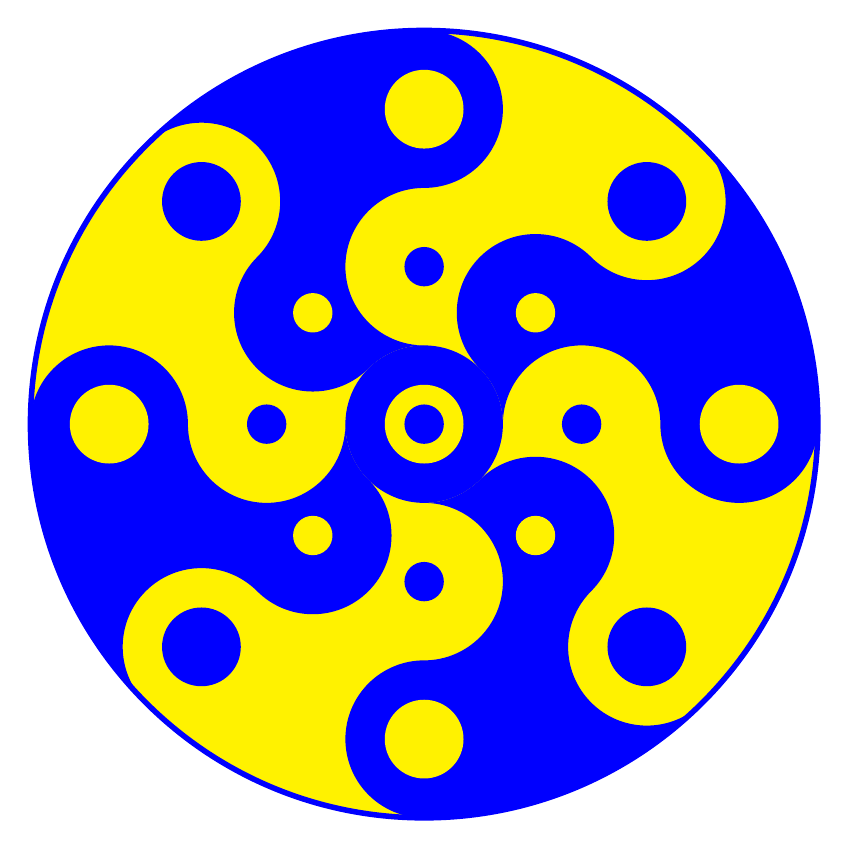
\begin{tikzpicture}
		\def\r{5}
		\pgfmathsetmacro{\rm}{\r/5}
		\pgfmathsetmacro{\rh}{\rm/2}
		\pgfmathsetmacro{\rb}{\rh/2}
		\colorlet{mau1}{blue}
		\colorlet{mau2}{yellow}
		\fill[mau2](0:0) circle (\r);
		\draw[mau1,line width=2] (0:0) circle (\r);
		\fill[mau1] (0:0) circle (\rm);
		\fill[mau2](0:0) circle (\rh);
		\fill[mau1](0:0) circle (\rb);
		\foreach \i in {1,...,4}{
			\pgfmathsetmacro{\quay}{\i *90}
			\fill[mau1,rotate=\quay] (0:\rm) arc(180:0:\rm) arc (180:360:\rm) arc(0:45:\r) arc(45:-135:\rm) arc(45:225:\rm) arc(45:0:\rm);
			\fill[mau2,rotate=\quay] (0:4*\rm) circle (\rh);
			\fill[mau1,rotate=\quay](0:2*\rm) circle (\rb);
		}
		\foreach \i in {1,...,4}{
			\pgfmathsetmacro{\quay}{\i *90-45}
			\fill[mau1,rotate=\quay] (0:4*\rm) circle (\rh);
			\fill[mau2,rotate=\quay](0:2*\rm) circle (\rb);
		}
	\end{tikzpicture}
\end{document}